% Chapter Template

\chapter{Software Architecture} % Main chapter title

\label{ChapterX} % Change X to a consecutive number; for referencing this chapter elsewhere, use \ref{ChapterX}

\lhead{\emph{Software Architecture}} % Change X to a consecutive number; this is for the header on each page - perhaps a shortened title

%----------------------------------------------------------------------------------------
%	SECTION 1
%----------------------------------------------------------------------------------------

\section{Version}

\begin{tabular}{| p{1.5cm} | p{2cm} | p{9cm} | p{1.5cm} |}
	\hline
	Version & Date 		& Change & Author \\ \hline
	0.1 	& 8.10.2014 		& Setup document  										& JR \\ \hline
	0.2 	& 12.10.2014		& Class diagrams										& JR \\ \hline
	0.3 	& 16.10.2014		& Text													& JR \\ \hline
	0.4 	& 20.10.2014		& Activity diagram										& JR \\ \hline
	1.0 	& 21.10.2014		& Grammar, Diagram fixes								& JR \\ \hline

\end{tabular}

\section{Introduction}

This document contains the description of the software architecture of the context extraction test framework. 

\pagebreak

\section{Data model}

The following diagram shows the data model of the application. 

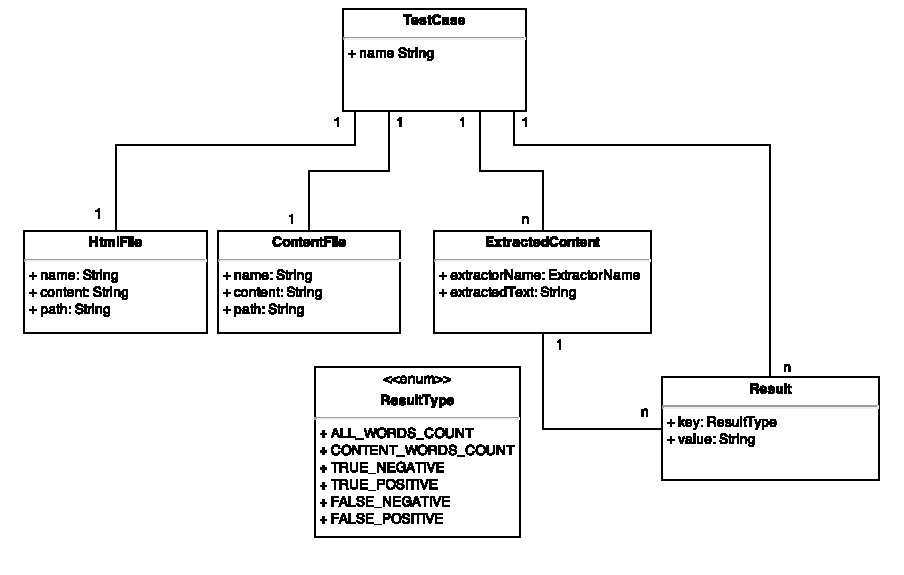
\includegraphics[width=14cm]{Figures/dataModel.pdf}


\subsection{TestCase}
A TestCase object is generated for each HTML/content file pair in the input folders. A TestCase has a a name which is unique and matches the name of the content and HTML file.

\subsection{HtmlFile}
Each TestCase has an HtmlFile object. It contains the content of the actual HTML file as String and the file path.

\subsection{ContentFile}
Each TestCase has a ContentFile object. It contains the content of the actual text file as String and the file path.

\subsection{ExctractedContent}
Each TestCase can have multiple ExctractedContent objects. Each of them represents a result of a content extraction from an extractor such as Justext or Boilerpipe.

\subsection{Result}
A TestCase or an ExctractedContent object can have Result objects. The results are key value pairs which represent analytical data. An example for a Result related to a TestCase would be the word count of the content file which is generally valid. An example for a Result related to an ExctractedContent would be the word count of true negative words which is only valid for one specific ExctractedContent.


\begin{landscape}

\section{Business Logic}

The following diagram shows the business logic of the application. The diagram does not show all of the classes but the most important ones. 

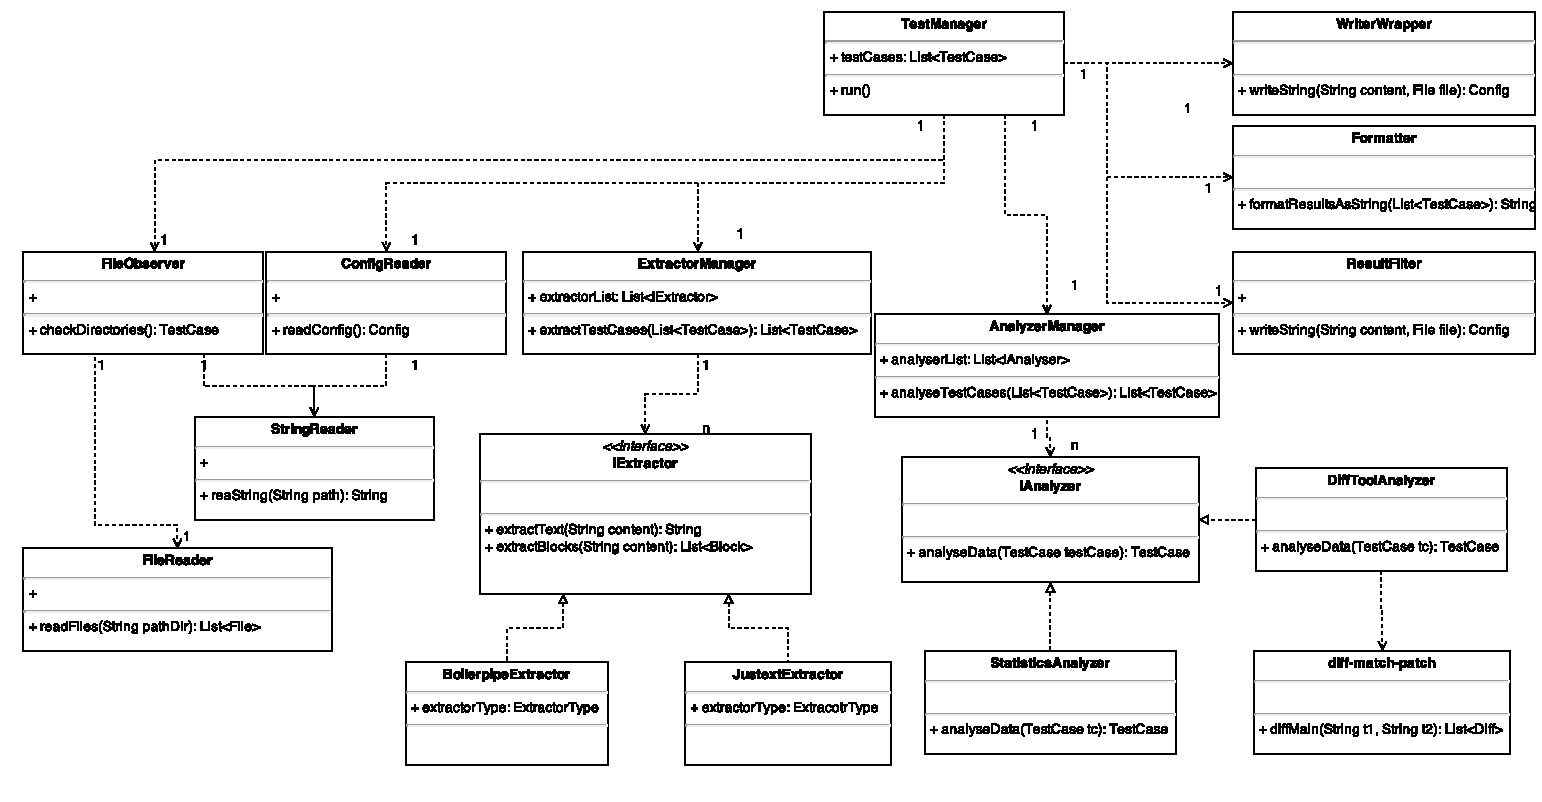
\includegraphics[width=23cm]{Figures/architecutre.pdf}

\end{landscape}

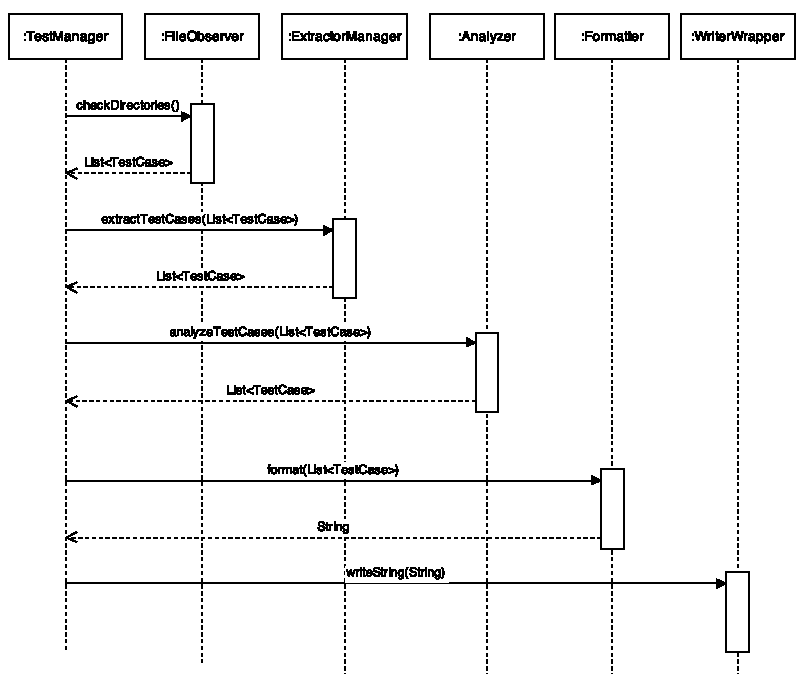
\includegraphics[width=15cm]{Figures/activityDiagram.pdf}
The data model is passed through the business logic and is enriched with data during the test procedure. First the input directories are checked for files by the FileObserver and TestCases are generated for each file pair with the same name. Then all the TestCases are then handed over to the ExtractorManager. The ExtractorManager extracts each TestCase with all available implementations of IExtractor and puts the Results into ExtractionResults. After that, all the TestCases are handed over to the Analyzer which runs each implementation of IAnalyzer. Each IAnalyzer produces at least one Result and puts it into the TestCase. To simplify the diagram, only two Analyzers are drawn. After generating some Results, the Formatter serializes the Result Objects into a String as a CSV table and the WriterWrapper persists the CSV data into an output file.



